\part{Entwurfsprozesse und Anforderungsanalyse}
\section{Entwicklungsprozess}
\subsection{}
\textbf{Was versteht man unter dem Begriff Phasenmodell?}
\begin{itemize}
    \item Partitionierung des Herstellungsprozesses
    \item Definierte abgegrenzte Phasen
    \item Vorgabe von Zwischenergebnissen
    \item Festlegung der Reihenfolge
\end{itemize}

\textbf{Nennen Sie ein Beispiel für ein Phasenmodell.In welche Phasen gliedert sich das von Ihnen gewählte
    Modell?}
\begin{figure}[H]
    \centering
    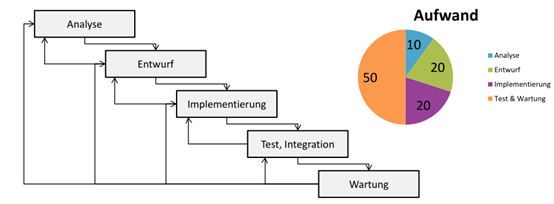
\includegraphics[width=.6\linewidth]{Graphics/Wasserfall-Modell.png}
    \caption{Wasserfall-Modell}
\end{figure}
Es gliedert sich in folgende Phasen:
\begin{enumerate}
    \item Analyse
    \item Entwurf
    \item Implementierung
    \item Test, Integration
    \item Wartung
\end{enumerate}

\subsection{}\textbf{Im V-Modell ’97 besteht der erste Schritt darin Anforderungen zu erstellen und festzulegen. Welche Quellen können dabei für die Erstellung von Anforderungen herangezogen werden?}
\begin{itemize}
    \item \begin{itemize}
              \item Prototypen
              \item Workshops
          \end{itemize}
    \item \begin{itemize}
              \item Supportmitarbeiter
              \item Untrainierte Nutzer
          \end{itemize}
    \item\begin{itemize}
              \item Feedback
              \item Fehlerberichte
              \item Interviews
          \end{itemize}
    \item Andere Systeme
\end{itemize}

\subsection{}
\textbf{Der Mensch ist ein schlechter Überwacher von automatisierten Systemen.}

\textbf{Welche Maßnahmen können den Menschen bei dieser Überwachungsaufgabe unterstützen?}
\begin{itemize}
    \item Anzeigen können dem Überwacher helfen, die Leistungsfähigkeit des Systems einzuschätzen
    \item Die Verantwortung zwiscen Überwacher und Fahrzeuge muss jederzeit geklärt sein\begin{itemize}
              \item Mögliches Kontrollvakuum
          \end{itemize}
    \item Ebenso muss die Kontrollmöglichkeit jederzeit eindeutig sein\begin{itemize}
              \item Möglicher Kontrollüberfluss
          \end{itemize}
\end{itemize}

\subsection{Evolutionäre Modelle}
\subsubsection{}
\textbf{Was zeichnet evolutionäre Modelle aus? }
\begin{figure}[H]
    \centering
    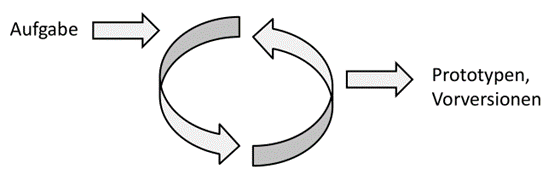
\includegraphics[width=.5\linewidth]{Graphics/Evolutional_Model.png}
    \caption{Evolutionäre Modelle}
\end{figure}
\begin{itemize}
    \item Kurz Iterationen immer derselben Phasen
    \item Erzeugung von Prototypen
\end{itemize}

\subsubsection{}
\textbf{Wofür sind diese Modelle primär geeignet?}

Gut geeignet für kleine Projekte mit unklaren Anforderungen

\subsection{V-Modells von ’97}
\textbf{In der Vorlesung haben Sie das V-Modells von ’97 kennengelernt.}
\subsubsection{}
\textbf{In welche vier Schritte gliedert sich der „linke Ast“ des Modells?}
\begin{figure}[H]
    \centering
    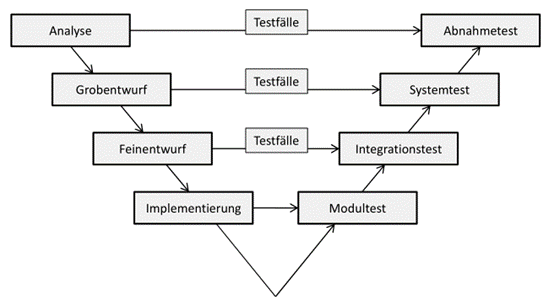
\includegraphics[width=.6\linewidth]{Graphics/V_Modell_97.png}
    \caption{V-Modell '97}
\end{figure}
\begin{enumerate}
    \item Anforderungsanalyse
    \item Grobenentwurf
    \item Feinentwurf
    \item Implementierung
\end{enumerate}
\subsubsection{}
\textbf{Was zeichnet die Schritte jeweils aus?}
\begin{enumerate}
    \item Analyse\begin{itemize}
              \item Kontext des Projekts definieren
              \item Anforderungen erstellen
              \item Eingabe: Lastenheft, Kunden
              \item Ausgabe: Kontextdiagramm, Anforderungen
          \end{itemize}
    \item Grobenentwurf\begin{itemize}
              \item Architekturentwurf
              \item Unabhängig von Programmiersprachen
              \item Funktionale Betrachtung/Systemarchitektur
              \item Eingabe: Ergebnis der Anforderungsanalyse, Projektkontext
              \item Ausgabe: Subsystem- und Schnittstellen-Spezifikation
          \end{itemize}
    \item Feinentwwurf\begin{itemize}
              \item Entwurf von\begin{itemize}
                        \item Komponenten
                        \item Datenstrukturen
                        \item Algorithmen
                    \end{itemize}
              \item Angepasst an Programmiersprache(n)
              \item Eingabe: Subsystem- und Schnittstellen-Spezifikation
              \item Ausgabe: Softwareentwurf, Testfälle
          \end{itemize}
    \item Implementierung\begin{itemize}
              \item Definition: Implementierung ist die Menge aller Tätigkeiten zur Umsetzung der gegebenen(technischen) Systemarchitektur und detallierten Spezifikation in ein lauffähiges, testbares, dokumentiertes Produkt.
              \item Eingabe: Subsystem- und Schnittstellen-Spezifikation, Softwareentwurf, Testfälle
              \item Ausgabe: lauffähiges Produkt, Testplanung, Dokumentation
          \end{itemize}
\end{enumerate}

\section{Agile Entwicklung}
\subsection{}
\textbf{Wie unterscheiden sich iterative und inkrementelle Entwicklung?}
\begin{itemize}
    \item Kurze Feedbackzyklen
    \item Entwicklerteamorientiert(Ergenverantwortung und -organisation, Kommunikation etc.)
    \item Qualitätsorientierung bereits zu Beginn
    \item Kontinuierliche Verbesserungen
\end{itemize}

\subsection{}
\textbf{Sie haben in der Vorlesung das Agile Manifest der Softwareentwicklung kennengelernt. Welches sind die vier Leitwerte dieses Manifests?}

\begin{center}
    \begin{minipage}{.48\linewidth}
        \begin{flushright}
            \textbf{Individuen und Interaktionen}

            \textbf{Funktionierende Software}

            \textbf{Zusammenarbeit mit dem Kunden}

            \textbf{Reagieren auf Veränderung}
        \end{flushright}
    \end{minipage}
    \begin{minipage}{.48\linewidth}
        \begin{flushleft}
            mehr als Prozesse und Werkzeuge

            mehr als umfassende Dokumentation

            mehr als Vertragsverhandlung

            mehr als das Befolgen eines Plans
        \end{flushleft}
    \end{minipage}
\end{center}


\subsection{}
\textbf{Welche agilen Prozesswerkzeuge bzw. Methoden findet besonders im Automotive-Bereich Anwendung?}
\begin{itemize}
    \item Scrum
    \item Continuous Integration
    \item Kanban
\end{itemize}

\subsection{}
\textbf{Was ist das primäre Ziel der agilen Methode der "Continuous Integration"\ und was zeichnet diese weiterhin aus?}
\subsubsection{Primäres Ziel}
Integrationsprobleme vermeiden
\subsubsection{Was zeichnet weiterhin aus}
\begin{itemize}
    \item Mindestens täglich Code einchecken
    \item Code muss vor dem Einchecken funktionieren
    \item Nicht einchecken, solange Integrationsprobleme vorliegen
    \item Verursacher müssen Integrationsprobleme umgehend beheben oder Änderungen rückgängig machen
\end{itemize}

\subsection{}
\textbf{Welche Nachteile hat die agile Entwicklung}
\begin{itemize}
    \item Skaliert nicht mit Aufgabenumfängen
    \item Verhindert langfristige Planung
    \item Feature-getrieben
\end{itemize}

\section{VSD(Value-Sensitive-Design)}
\subsection{}
\textbf{Was versteht man unter dem Paradigma des Value-Sensitive-Design}

Menschlicher Werte in der Entwicklung

Ansatz:
\begin{itemize}
    \item Identifikation aller direkten und indirekten Stakeholder
    \item Identifikation der relevanten Werten der Stakeholder
    \item Berücksichtung der Werte in allen Prozessschritten der Entwicklung
\end{itemize}
\subsection{}
\textbf{Aus welchen drei Bestandteilen setzt sich die integrative und iterative Methodik des Value-Sensitive-Design zusammen? Was zeichent diese Bestandteile aus?}
\begin{itemize}
    \item Konzeptuelle Investigationen\begin{itemize}
              \item Wer sind Stakeholder?
              \item Was sind relevante Werte?
              \item Gibt es Trade-offs/Hierarchien?
          \end{itemize}
    \item Empirische Investigationen\begin{itemize}
              \item Sozialwissenschaftliche Methoden: Kennen wir alle Stakeholder und ihre Werte?
          \end{itemize}
    \item Technische Investigationen\begin{itemize}
              \item Was beeinflusst die Implementierung verschiedene Werte?
          \end{itemize}
\end{itemize}

\section{Anforderungen}
\subsection{}
\textbf{In welche Aufgaben gliedert sich das Anforderungsmanagement?}
\begin{enumerate}
    \item Anforderungsmanagement planen und steuern
    \item Anfangspunkt setzen
    \item Anforderungen erheben
    \item Anforderungen dokumentieren
    \item Anforderungen qualitätssichern
    \item Anforderungen verwalten
\end{enumerate}
\subsection{}
\textbf{Warum ist Anforderungsmanagement erforderlich?}

Anforderungsmanagement
\begin{itemize}
    \item dient der Kommunikation und Einigung zwischen allen Beteiligten
    \item bildet die Basis der Kalkulation
    \item ist Vertragsbestandteil zwischen Auftraggeber und Auftragnehmer
    \item ist die Vorgabe für die Entwickler
    \item bildet dis Basis für Testfälle
    \item ermöglicht frühzeitige Erkennung von Problemen
    \item dient der Interessenvertretung der Endanwender
\end{itemize}
$\rightarrow$ stellt Produkterfolg sicher
\subsection{}
\textbf{Wie sollte in eine Anforderung aufgabaut sein?}
\begin{figure}[H]
    \centering
    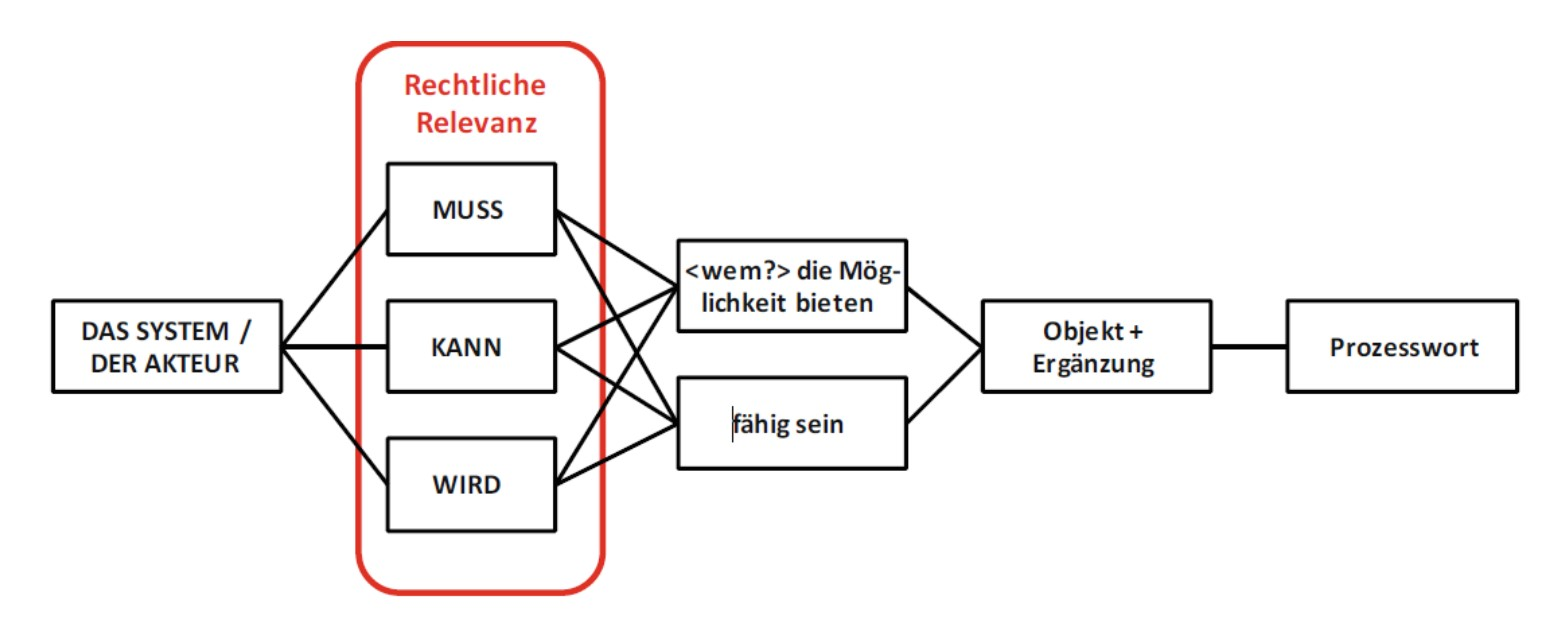
\includegraphics[width=.8\linewidth]{Graphics/Anforderung_Aufbau.jpg}
    \caption{Aufbau einer Anforderung}
\end{figure}